\section{Graph and network optimization}

\subsection{Graphs}

\subsubsection{Definitions and characteristics}

In the following section we will explain some basic concepts about the graphs. The terms used are important, and we will use the definition box to highlight these words.

\highspace
\begin{definitionbox}[: graph]
    A \definitionWithSpecificIndex{graph}{Graph} is a pair $G = \left(N,E\right)$, with $N$ a set of \textbf{nodes} or \textbf{vertices} and $E \subseteq N \times N$ a set of \textbf{edges} or \textbf{arcs} connecting them pairwise.
\end{definitionbox}

\highspace
\begin{definitionbox}[: edge]
    An \definitionWithSpecificIndex{edge}{Edge} connecting the nodes $i$ and $j$ is represented by
    \begin{itemize}
        \item Graph undirected: $\left\{i,j\right\}$
        \item Graph directed: $\left(i,j\right)$
    \end{itemize}
\end{definitionbox}

\highspace
\begin{examplebox}
    For \example{example}, a road network which connects $n$ cities can be modelled, by a graph where a city corresponds to a node, and a connection corresponds to an edge.

    \begin{center}
        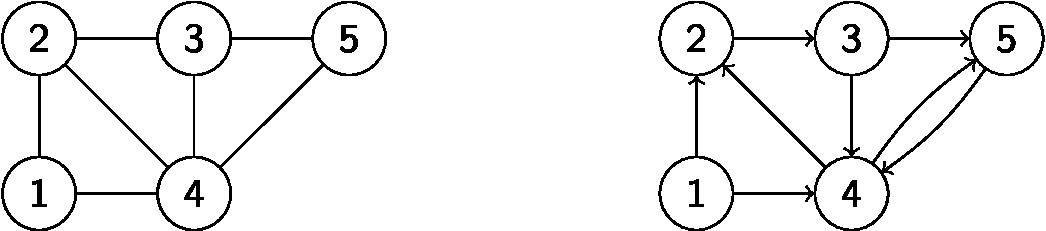
\includegraphics[width=.8\textwidth]{img/graphs-1.pdf}
    \end{center}

    \noindent
    \begin{itemize}
        \item Undirected graph:
        \begin{itemize}
            \item $N = \left\{1,2,3,4,5\right\}$
            \item $E = \left\{
                \left\{1,2\right\},
                \left\{1,4\right\},
                \left\{2,3\right\},
                \left\{2,4\right\},
                \left\{3,4\right\},
                \left\{3,5\right\},
                \left\{4,5\right\}
            \right\}$
        \end{itemize}
        
        \item Directed graph:
        \begin{itemize}
            \item $N = \left\{1,2,3,4,5\right\}$
            \item $E' = \left\{
                \left(1,2\right),
                \left(1,4\right),
                \left(2,3\right),
                \left(2,4\right),
                \left(3,4\right),
                \left(3,5\right),
                \left(4,5\right)
            \right\}$
        \end{itemize}
    \end{itemize}
\end{examplebox}

\newpage

\noindent
Some graph properties are:
\begin{itemize}
    \item Two \textbf{nodes} are \definitionWithSpecificIndex{adjacent}{Adjacent nodes} if they are \textbf{connected by an edge}.

    \item An \textbf{edge} $e$ is \definitionWithSpecificIndex{incident}{Incident edge} in a node $v$ if $v$ is an endpoint of $e$.
    
    In other words, in a graph $G$, two edges are incident \textbf{if they share a common vertex}. For example, edge $E_{1}=\left(v_{1}, v_{2}\right)$ and edge $\left(v_{1}, v_{3}\right)$ are incident as they share the same vertex $v_{1}$.

    \item The degree concept depends on the type of graph:
    \begin{itemize}
        \item Undirected graph: the \definitionWithSpecificIndex{degree}{Node degree} of a node is the \textbf{number of incident edges}.

        \item Directed graph: the \definitionWithSpecificIndex{in-degree}{Node in-degree} and \definitionWithSpecificIndex{out-degree}{Node out-degree} of a node is the \textbf{number of arcs that have it as succesor} and \textbf{predecessor}.
    \end{itemize}
\end{itemize}

\highspace
\begin{examplebox}[: adjacent, incident, degree, in-degree and out-degree]
    Given the graphs:
    
    \begin{center}
        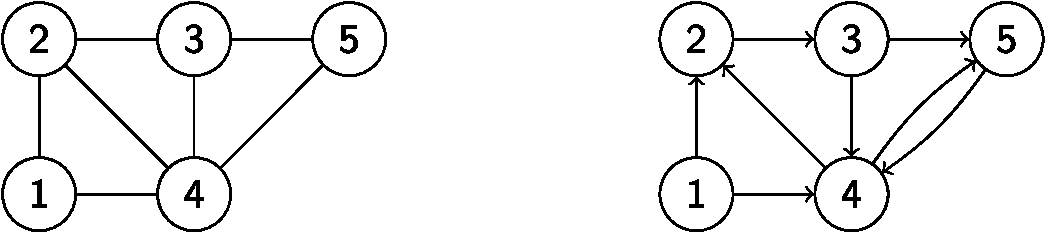
\includegraphics[width=.8\textwidth]{img/graphs-2.pdf}
    \end{center}

    \begin{itemize}
        \item Undirected graph:
        \begin{itemize}
            \item Nodes 1 and 2 are \textbf{adjacent} (unlike nodes 1 and 3).
            \item Edge $\left\{1,2\right\}$ is \textbf{incident} in nodes 1 and 2.
            \item Node 1 has \textbf{degree} 2, node 4 has \textbf{degree} 4.
        \end{itemize}

        \item Directed graph: node 1 has \textbf{in-degree} 0, and \textbf{out-degree} 2.
    \end{itemize}
\end{examplebox}

\highspace
Other useful features include:
\begin{itemize}
    \item A \definitionWithSpecificIndex{(directed) path from $i \in N$ to $j \in N$}{Directed path from $i \in N$ to $j \in N$} is a sequence of (arcs) edges:
    \begin{equation*}
        p = \left\langle \left\{v_{1}, v_{2}\right\}, \left\{v_{2}, v_{3}\right\}, \dots, \left\{v_{k-1}, v_{k}\right\} \right\rangle
    \end{equation*}
    Connecting nodes $v_{1}$ and $v_{k}$, with $\left\{v_{i}, v_{i+1}\right\} \in E$, for $i = 0, \dots, k-1$.

    \item A generic \textbf{node} $u$ and $v$ are \definitionWithSpecificIndex{connected}{Connected nodes} if there is a path connecting them.
    
    \item A \textbf{graph} $\left(N,E\right)$ is \definitionWithSpecificIndex{connected}{Connected graph} if two generic nodes $u,v$ are connected, $\forall u,v \in N$. Recall that in generic graph notation, the variable $N$ represents a set of nodes or vertices and $E$ represents a set of edges or arcs connecting them in pairs.
    
    \item A \textbf{graph} $\left(N,E\right)$ is \definitionWithSpecificIndex{strongly connected}{Strongly connected graph} if two generic nodes $u,v$ are connected by a directed path, $\forall u,v \in N$ (for any node in the set of nodes or vertices of the graph).
\end{itemize}

\highspace
\begin{examplebox}[: directed path, connected nodes, connected graph, strongly connected]
    Given the graphs:
    
    \begin{center}
        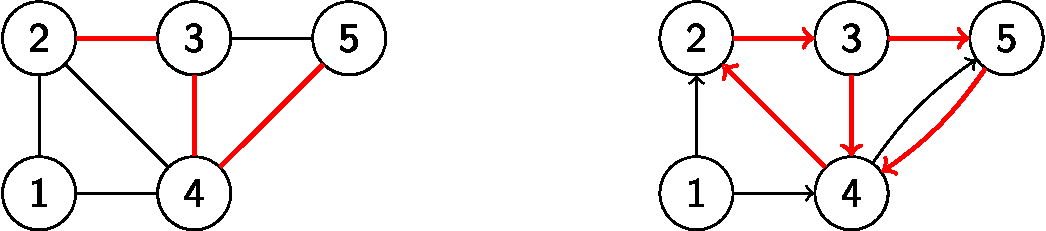
\includegraphics[width=.8\textwidth]{img/graphs-3.pdf}
    \end{center}

    \begin{itemize}
        \item Undirected graph:
        \begin{itemize}
            \item $\left\langle \left\{2,3\right\}, \left\{3,4\right\}, \left\{4,5\right\} \right\rangle$ is a \textbf{path} from node 2 to node 5.
            \item \textbf{Nodes} 2 and 5 are \textbf{connected}.
            \item It is a \textbf{connected graph}.
        \end{itemize}

        \item Directed graph:
        \begin{itemize}
            \item $\left\langle \left\{3,5\right\}, \left\{5,4\right\}, \left\{4,2\right\}, \left\{2,3\right\}, \left\{3,4\right\} \right\rangle$ is a \textbf{directed path} from node 3 to node 4.
            
            \item It is not a \textbf{strongly connected graph} because the node 1 cannot be the destination of none path. In other words, doesn't exist a directed path from node $u$ to node $1$ (where $u$ is a generic node, $\forall u \in N \setminus \left\{1\right\}$).
        \end{itemize}
    \end{itemize}
\end{examplebox}

\highspace
Finally, there are other interesting properties and notations about graphs and edges:
\begin{itemize}
    \item A \definitionWithSpecificIndex{cycle (circuit)}{Cycle in graph}\index{Circuit in graph} is a directed path with $v_{1} = v_{k}$ (source and destination are the same).

    \item A \textbf{graph} is \definitionWithSpecificIndex{bipartite}{Bipartite graph} if there is a partition $N = N_{1} \cup N_{2}$ $\left(N_{1} \cap N_{2} = \emptyset\right)$ such that no edge connects nodes in the same subset.

    \item A \textbf{graph} is \definitionWithSpecificIndex{complete}{Complete graph} if $E = \left\{\left\{v_{j}, v_{j}\right\} \: : \: v_{i}, v_{j} \in N \: \land \: i \le j\right\}$.

    \item Given a directed graph $G = \left(N,A\right)$ and $S \subset N$, the \definitionWithSpecificIndex{outgoing cut}{Outgoing cut} induced by $S$ is:
    \begin{equation*}
        \delta^{+}\left(S\right) = \left\{\left(u,v\right) \in A \: : \: u \in S \: \land : v \in N \subseteq S\right\}
    \end{equation*}
    The \definitionWithSpecificIndex{incoming cut}{Incoming cut} induced by $S$ is:
    \begin{equation*}
        \delta^{-}\left(S\right) = \left\{\left(u,v\right) \in A \: : \: v \in S \: \land : u \in N \subseteq S\right\}
    \end{equation*}
\end{itemize}

\newpage

\begin{examplebox}[: cycle/circuit in graph, bipartite graph, complete graph, out/incoming cut]
    An example of cycle in graph:
    
    \begin{center}
        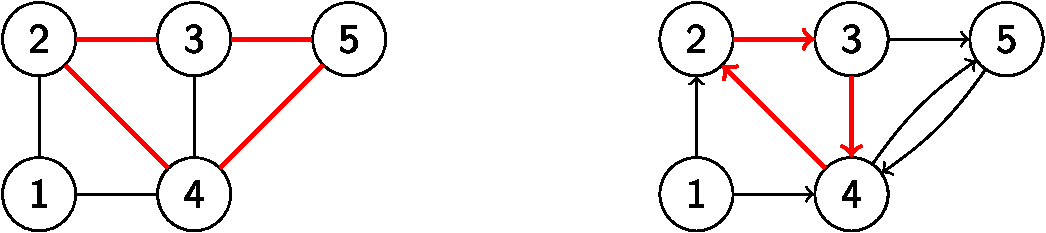
\includegraphics[width=.8\textwidth]{img/graphs-4.pdf}
    \end{center}

    \begin{itemize}
        \item Undirected graph: $\left\langle \left\{2,3\right\}, \left\{3,5\right\}, \left\{5,4\right\}, \left\{4,2\right\} \right\rangle$ is a cycle.
        \item Directed graph: $\left\langle \left(2,3\right), \left(3,4\right), \left(4,2\right) \right\rangle$ is a circuit.
    \end{itemize}
    %
    %

    An example of bipartite/complete graph:

    \begin{center}
        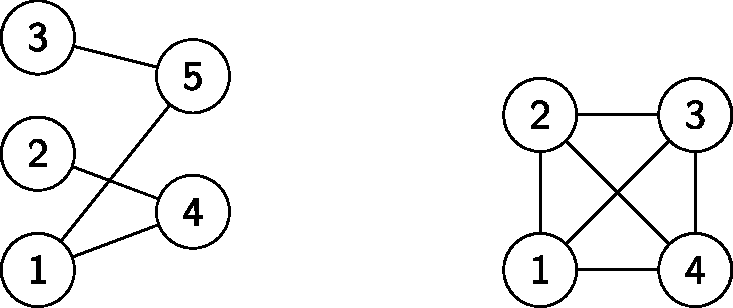
\includegraphics[width=.6\textwidth]{img/graphs-5.pdf}
    \end{center}

    \begin{itemize}
        \item To the left a \textbf{bipartite graph}, because:
        \begin{equation*}
            N_{1} = \left\{1,2,3\right\} \hspace{2em} N_{2} = \left\{4,5\right\}
        \end{equation*}
        \item And to the right a \textbf{complete graph}.
    \end{itemize}
    %
    %

    Finally, an example of out/incoming cut:
    
    \begin{center}
        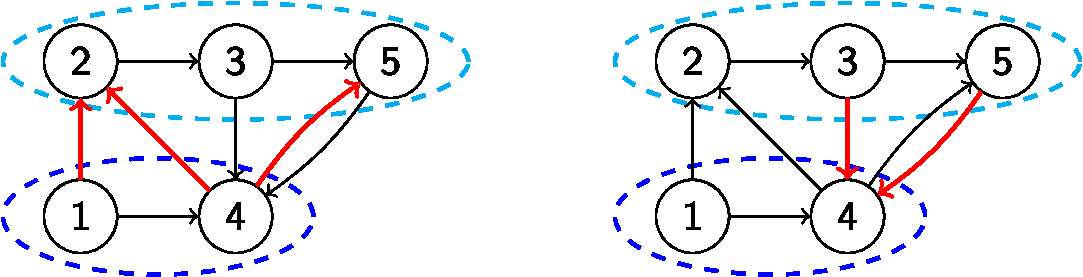
\includegraphics[width=.8\textwidth]{img/graphs-6.pdf}
    \end{center}

    \begin{itemize}
        \item Left graph: 
        \begin{equation*}
            \begin{array}{rcl}
                \delta^{+}\left(\left\{1,4\right\}\right) &=& \left(\left\{1,2\right\}, \left\{4,2\right\}, \left\{4,5\right\}\right) \\ [.5em]
                S &=& \left\{1,4\right\} \\ [.5em]
                N \setminus S &=& \left\{2,3,5\right\}
            \end{array}
        \end{equation*}

        \item Right graph: 
        \begin{equation*}
            \begin{array}{rcl}
                \delta^{-}\left(\left\{1,4\right\}\right) &=& \left(\left\{3,4\right\}, \left\{5,4\right\}\right) \\ [.5em]
                S &=& \left\{1,4\right\} \\ [.5em]
                N \setminus S &=& \left\{2,3,5\right\}
            \end{array}
        \end{equation*}
    \end{itemize}
\end{examplebox}

\subsubsection{Graphical representation}

Such a matrix can easily be represented as a graph. This guarantees that it can be stored efficiently in a computer. But to understand how to do this in general, it's important to understand some other important properties:
\begin{itemize}
    \item For any graph $G$ with $n$ nodes, the \textbf{number of edges} satisfies:
    \begin{itemize}
        \item $m \le \dfrac{n\left(n-1\right)}{2}$ if $G$ is undirected.
        \item $m \le n\left(n-1\right)$ if $G$ is directed.
    \end{itemize}

    \item A graph is \definitionWithSpecificIndex{dense}{Dense graph} if $m \approx n^{2}$ and \definitionWithSpecificIndex{sparse}{Sparse graph} if $m \ll n^{2}$. Where $m$ is the number of arcs and $n$ the number of nodes.

    \item For dense directed graphs, exist an \textbf{adjacency matrix} $A_{n \times n}$:
    \begin{equation*}
        \begin{cases}
            a_{ij} = 1 & \text{if } \left(i,j\right) \in A \\
            a_{ij} = 0 & \text{otherwise}
        \end{cases}
    \end{equation*}
\end{itemize}
To build the adjacency matrix it is necessary to create a \textbf{list of successors} for each node. In other words, for \textbf{each node} we need to write the \textbf{outgoing edges} and write the matrix.
\begin{equation*}
    A = \begin{bmatrix}
        0 & 1 & 0 & 1 & 0 \\
        0 & 0 & 1 & 0 & 0 \\
        0 & 0 & 0 & 1 & 1 \\
        0 & 1 & 0 & 0 & 1 \\
        0 & 0 & 0 & 1 & 0
    \end{bmatrix}
    \hspace{2em}
    \begin{array}{rcl}
        S\left(1\right) &=& \left\{2,4\right\} \\
        S\left(2\right) &=& \left\{3\right\} \\
        S\left(3\right) &=& \left\{4,5\right\} \\
        S\left(4\right) &=& \left\{2,5\right\} \\
        S\left(5\right) &=& \left\{4\right\}
    \end{array}
\end{equation*}
Each row represents a node, and we set the value 1 if the column index is a node that has the arc of the row node as its incoming edge. So row one (node one) has the value one in column two (node two) and column four (node four).

\longline

\subsubsection{Graph reachability problem}

In general the \definitionWithSpecificIndex{graph reachability problem}{Graph reachability problem} can be formulated as follows.

\begin{definitionbox}[: graph reachability problem]
    Given a directed graph $G = \left(N,A\right)$ and a node $s$, determine all the node that are reachable from $s$.
\end{definitionbox}

\noindent
Where $N$ is the set of nodes and $A$ is the set of edges.

\highspace
The problem takes:
\begin{itemize}
    \item As \textbf{input} a \emph{\textbf{graph}} $G = \left(N,A\right)$ described by the successor lists and node $s \in N$.
    
    \item As \textbf{output} produces a \emph{\textbf{subset}} $M \subseteq N$ \emph{\textbf{of nodes}} of the graph $G$ reachable from $s$.
\end{itemize}
Our goal is to devise an efficient algorithm that allows us to find all nodes reachable from $s$.

\newpage

\paragraph{Description and algorithm}

\begin{definitionbox}[: Breadth-First Search]
    \definition{Breadth-First Search (BFS)} is an \textbf{algorithm for searching a tree data structure for a node that satisfies a given property}. It starts at the tree root and explores all nodes at the present depth prior to moving on to the nodes at the next depth level. Extra memory, usually a queue, is needed to keep track of the child nodes that were encountered but not yet explored.
\end{definitionbox}

\begin{lstlisting}[language=pseudo-code, caption={Graph reachability problem: Breadth-First Search $O\left(\left|N\right|+\left|A\right|\right)$}]
Q $\leftarrow$ $\{$s$\}$; $\label{bfs: q-definition}$
M $\leftarrow$ $\emptyset$; $\label{bfs: m-definition}$
while Q $\ne$ $\emptyset$ do: $\label{bfs: while cycle}$
    u $\leftarrow$ node in Q; $\label{bfs: take an element from the queue}$
    Q $\leftarrow$ Q $\setminus$ $\{$u$\}$; $\label{bfs: remove the popped item from the queue}$
    // label u
    M $\leftarrow$ M $\cup$ $\{$u$\}$ $\label{bfs: labeled as explored}$
    for (u, v) $\in$ $\delta^{+}$ (u) do: $\label{bfs: for each tuple in outgoing cut}$
        if v $\notin$ M and v $\notin$ Q: $\label{bfs: if adjacent node is not in reachable set and not in the queue}$
            Q $\leftarrow$ Q $\cup$ $\{$v$\}$ $\label{bfs: add the node v to the queue}$
\end{lstlisting}

\begin{itemize}
    \item[Rows \ref{bfs: q-definition}-\ref{bfs: m-definition}.] Declare a queue \texttt{Q} containing the nodes reachable from the source \texttt{s} and \textbf{not yet processed}. It is managed as a FIFO (First-In First-Out) queue. By definition, we add the \texttt{s} node at the beginning because it is our entry point.
    
    Then we declare the set \texttt{M}. It represents the subset of nodes of the graph that are reachable from the source \texttt{s}. Obviously, it is empty at the beginning of the algorithm.

    \item[Row \ref{bfs: while cycle}.] The BFS algorithm continues to process the nodes until the queue is empty. As long as there is an element, it continues.
    
    \item[Rows \ref{bfs: take an element from the queue}-\ref{bfs: remove the popped item from the queue}.] Take a node from the queue \texttt{Q} and assign it to the variable \texttt{u}. Also remove the element \texttt{u} from the set \texttt{Q}. In other words, perform a difference operation between the sets \texttt{Q} and the set composed only of the element \texttt{u} ($\texttt{Q} \setminus \left\{\texttt{u}\right\}$).
    
    For example, in Python we can get the same result using the \href{https://docs.python.org/3/library/collections.html#collections.deque.popleft}{\texttt{popleft}} method of the \href{https://docs.python.org/3/tutorial/datastructures.html#using-lists-as-queues}{\texttt{deque} data structure}.

    \item[Row \ref{bfs: labeled as explored}.] Using the union between sets, add the visited node \texttt{u} to the subset \texttt{M} of reachable nodes. This operation is also called \dquotes{labeling} because you are \emph{labeling} a node as \emph{visited}.
    
    \item[Row \ref{bfs: for each tuple in outgoing cut}.] Iterate each tuple (node \texttt{u} just popped from the queue, node \texttt{v} adjacent to node \texttt{u}) in the outgoing cut set of node \texttt{u}.
    
    \item[Rows \ref{bfs: if adjacent node is not in reachable set and not in the queue}-\ref{bfs: add the node v to the queue}.] If the adjacent node \texttt{v} is not in the reachable set \texttt{M} and it is not in the queue (so it is not waiting to be evaluated), add the adjacent node \texttt{v} to \texttt{Q} using the union set operation.
\end{itemize}
As we said, the algorithm continues until the queue is not empty. Note that the queue is updated each time a neighboring node is found that is not already in the solution set (\texttt{M}).

\newpage

\paragraph{Complexity of algorithm}

\begin{flushleft}
    \textcolor{Green3}{\faIcon{clock} \textbf{BFS Algorithm - Time Complexity}}
\end{flushleft}
The BFS time complexity%
\footnote{In theoretical computer science, the time complexity is the computational complexity that describes the amount of computer time it takes to run an algorithm. Time complexity is commonly estimated by counting the number of elementary operations performed by the algorithm, supposing that each elementary operation takes a fixed amount of time to perform. Thus, the amount of time taken and the number of elementary operations performed by the algorithm are taken to be related by a constant factor. (\href{https://en.wikipedia.org/wiki/Time_complexity}{source})}
can be expressed as $O\left(\left|N\right|+\left|A\right|\right)$, since \textbf{every node and every edge will be explored in the \underline{worst case}}.
\begin{itemize}
    \item $\left|N\right|$ is the number of \textbf{nodes};
    \item $\left|A\right|$ is the number of \textbf{edges} in the graph.
\end{itemize}
Note that $O\left(\left|A\right|\right)$ may vary between $O\left(1\right)$ and $O\left(N^{2}\right)$, depending on how sparse the input graph is. For example, for \textbf{dense graphs}, exactly $O\left(N^{2}\right)$.

\highspace
\begin{flushleft}
    \textcolor{Green3}{\faIcon{memory} \textbf{BFS Algorithm - Space Complexity}}
\end{flushleft}
When the number of nodes (or vertices) in the graph is known ahead of time, and additional data structures are used to determine which vertices have already been added to the queue, the space complexity%
\footnote{The space complexity of an algorithm or a data structure is the amount of memory space required to solve an instance of the computational problem as a function of characteristics of the input. It is the memory required by an algorithm until it executes completely. This includes the memory space used by its inputs, called input space, and any other (auxiliary) memory it uses during execution, which is called auxiliary space. (\href{https://en.wikipedia.org/wiki/Space_complexity}{source})}
can be expressed as $O\left(\left|N\right|\right)$, where $\left|N\right|$ is the number of vertices. This is in addition to the space required for the graph itself, which may vary depending on the graph representation used by an implementation of the algorithm.

\highspace
In other words, the algorithm needs:
\begin{itemize}
    \item The \textbf{space to store} the set $N$, i.e. the \textbf{set of all nodes} in the graph.
    \item The \textbf{space to store the graph itself} depends on the implementation used.
\end{itemize}